\chapter{Android jako system operacyjny}

Android – według wiadomości zawartych w Wikipedii – to system operacyjny z jądrem Linux, przeznaczony dla urządzeń mobilnych, takich jak telefony komórkowe, smartfony, tablety (tablety PC) i netbooki. Według portalu AntyWeb.pl w maju 2015 roku system ten miał największy udział w rynku urządzeń mobilnych w Polsce, a wartość tego udziału od 2014 roku to około 65 %. 

\begin{figure}[!htb]
    \centering
    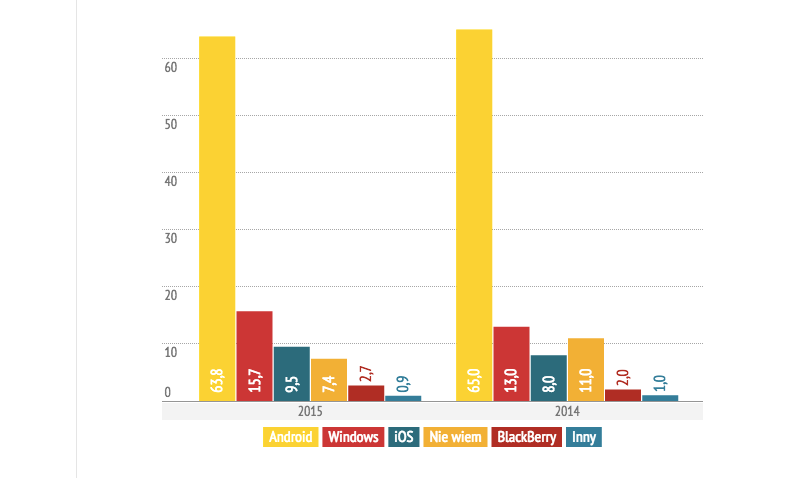
\includegraphics[width=15cm]{imgs/ch2_android_udzial_1.png}
    \caption
{Android – udział w rynku urządzeń mobilnych w Polsce. (Źródło: portal AntyWeb.pl, 05/2015)}
    \label{fig:android_udzial_polska}
\end{figure} 

Drugie miejsce, według tego samego portalu, zajmuje system Windows, a trzecie iOS. Na świecie proporcje udziału są nieco inne, ale ciągle na czele jest system Android, z wynikiem ponad 53\%, natomiast tutaj na drugim miejscu plasuje się już wyraźnie iOS z niemal 40-procentowym udziałem w rynku.

\begin{figure}[!htb]
    \centering
    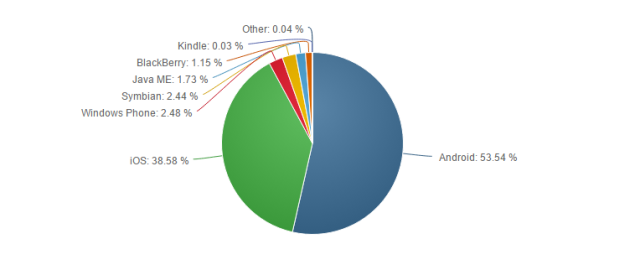
\includegraphics[width=17cm]{imgs/ch2_android_udzial_2.png}
    \caption
{Android – udział w rynku urządzeń mobilnych na świecie. (Źródło: portal android.com.pl, 09/2015)}
    \label{fig:android_udzial_zagranica}
\end{figure} 

Jako system operacyjny dostępny nieodpłatnie, Android zrzesza przy sobie dużą społeczność deweloperów piszących aplikacje, które poszerzają funkcjonalność urządzeń. W sierpniu 2014 roku w Google Play (wcześniej Android Market), dostępnych było ponad 1,3 miliona aplikacji, zarówno komercyjnych, jak i darmowych.

Najpopularniejszymi językami programowania, w których piszemy aplikacje na Androida, są Java i C++ ze środowiskiem Android NDK. O ile język Java wydawać się może najrozsądniejszym wyborem na pierwszy rzut oka, o tyle wielu programistów używa również środowiska NDK. Jest to zestaw narzędzi, który pozwala realizować części swojej aplikacji za pomocą kodu macierzystego języków takich jak C i C ++. Zazwyczaj środowisko to wykorzystuje się w celu pisania programów, które intensywnie wykorzystują CPU, takich jak silniki gier, przetwarzania sygnału i symulacji fizyki. Jednak deweloperzy muszą wziąć pod uwagę również wady takiego rozwiązania, które mogą nie do końca zbilansować korzyści. Natywny kod Androida na ogół nie powoduje zauważalnej poprawy wydajności, ale za to zawsze znacznie zwiększa złożoność aplikacji, który to problem i tak już jest dużym wyzwaniem dla programistów Java, co przybliżę w kolejnych rozdziałach. Podsumowując, z NDK należy korzystać tylko wtedy, jeśli uznamy, że jest to niezbędne dla wytwarzanej aplikacji, a nie dlatego, że lepiej czujemy się programując w języku C/C++. Zanim zdecydujemy się na to rozwiązanie, najpierw należy sprawdzić, czy androidowe API zapewnia funkcjonalność, której potrzebujemy.

Java i C czy C++ to jednak nie wszystkie języki, których możemy użyć przy programowaniu aplikacji na Androida. Podczas szukania materiałów do tej pracy spotkałem się z przykładami aplikacji napisanych w C\#, Delphi, czy nawet PHP. Stanowią one tak mały procent, że postanowiłem nie brać ich pod uwagę analizując opisywany problem testowalności oprogramowania na ten system operacyjny.


%tutaj przykłady jak użyć poszczególnych konstrukcji
%Przykładowy rysunek \ref{fig:sample_figure}. Prztykładowa tabela %\ref{tab:sample_table}. Przykładowy odnośnik do bibliografi \cite{bib:kowalski_2015}. \textbf{Powodzenia!}


%\begin{figure}[!htb]
%    \centering
%    \includegraphics[width=10cm]{imgs/sample_figure.jpg}
%    \caption{Przykłady rysunek}
%    \label{fig:sample_figure}
%\end{figure} 

%\begin{table}[]
%\centering
%\caption{Przykładowa tabela}
%\label{tab:sample_table}
%\begin{tabular}{|l|l|}
%\hline
%\textbf{Nazwa} & \textbf{Wartość} \\ \hline
%Test           & 1.2              \\ \hline
%Kwiatek        & 5                \\ \hline
%\end{tabular}
%\end{table}